\documentclass{jdf}

\begin{document}
Section: PUBP-6727
\title{Mutual Monitoring in the Cloud}
\author{Alexander Stein}

\maketitle
\thispagestyle{fancy}


\section*{Problem Statement}

Cloud computing infrastructure is essentially ubiquitous, but adoption is not without challenges. Cloud service providers must cater to customers in regulated sectors, complying with cybersecurity frameworks that create high barriers to entry. One barrier is ongoing evaluation of the provider's cybersecurity posture, often resulting in centralized bureaucracies. FedRAMP oversees and documents a prominent example of such a program, the Continuous Monitoring Program.

Are these bureaucracies an optimal solution, or a last resort that fails to keep pace with cloud technology as it proliferates and evolves? If they are a last resort, is there a better way?

\section*{Solution Statement}

I will use this research to design and evaluate an alternative to centralized continuous monitoring, mutual monitoring. The foundation of mutual monitoring will be federated data services, known in other security use cases as transparency services. The services will necessarily change cloud service provider and customer behavior, while also incentivizing auditors to sell value-add analytics services in these data services, and possibly obsolete centralized authorities like FedRAMP.

\section*{Completed Tasks (Last 2 Weeks)}

\begin{enumerate}
    \item I presented a proposal and reviewed scope of research with four advisors that are highly familiarity with FedRAMP strategy, policies, and operations. Three advisors have accepted, while one's acceptance is still pending.
    \item I began an outline for critical analysis for FedRAMP's centralized continuous monitoring model (\hyperlink{https://github.com/aj-stein/practicum_proposal/blob/main/paper.pdf}{e.g. proposal deliverable \#1}).
    \item I initialized a \hyperlink{https://github.com/aj-stein/conmotion.git}{code repository} to save the architecture documents and prototype code in version control (e.g. \hyperlink{https://github.com/aj-stein/practicum_proposal/blob/main/paper.pdf}{proposal deliverables \#3 and \#4}, respectively).
    \item I incorporate feedback from Professor Kuerbis into to add and adjust research topics and evaluation methods in my \hyperlink{https://github.com/aj-stein/practicum/blob/main/notes.pdf}{outline for the project and specific deliverables}.
    \begin{itemize}
        \item How is mutual monitoring different from continuous assessment?
        \item Are machine-readable compliance artifact's like NIST OSCAL related, competing, or complimentary?
        \item Do cloud providers currently assess and monitor one another? How?
        \item What are the incentives to expose posture data in a peer-to-peer model?
        \item What mechanisms and disincentives prevent abuse or manipulation?
    \end{itemize}
\end{enumerate}

\section*{Tasks for the Next Project Report}

In the next two weeks, I will focus on the following goals. I have sorted them in order of priority.

\begin{enumerate}
    \item Complete first draft of federated data service architecture, request feedback from advisors.
    \item Implement primary component of data service, submission API for cloud service providers and external third-party auditors.
    \item Complete outline of FedRAMP critical analysis.
    \item Start draft of FedRAMP critical analysis, request feedback from advisors.
\end{enumerate}

\section*{Questions or issues I'm having}

\subsection*{Alignment with Practicum Requirements}

\begin{enumerate}
    \item My project focuses on a policy challenge in cloud security, but does not have a conventional policy recommendation like other policy track proposals. Is a policy document an explicit requirement?
\end{enumerate}

\subsection*{Project Scope}

\begin{enumerate}
    \item One of my deliverables (a critical analysis of FedRAMP's current approach) is ancillary, but will establish important qualitative background. Should I include this deliverable in the final project appendix or use it as an input for a summary analysis in the final report only?
    \item One of my deliverables will be a prototype of federated data service, which will have server and client components that does statistical analysis of data without a user-friendly web interface to keep scope focused and the timeline reasonable?
    \item If I cannot complete all the code for the prototype and I must scope down the prototype and describe the future to keep to my proposed schedule, will this negatively impact my final grade for this project or is this normal?
\end{enumerate}

\subsection*{Evaluation and Measurement}

\begin{enumerate}
    \item I am proposing a novel solution that is considerably different from the current state, and the latter is not easily measurable. (It is also why I think the problem is important.) However, direct comparison is difficult. Is there any significant risk to my project if I design quantitative and qualitative metrics?    
\end{enumerate}

\section*{Methodology Paragraph Summary}

\section*{Timeline}

\begin{table}[h]
\begin{tabularx}{\textwidth}{|l|X|l|}
    \hline
    Week \# & Description of Task & Status \\ [0.5ex] 
    \hline
    W1 & Initialize code repository for prototype service & Complete \\
    \hline
    W1 & Present proposal to advisors and integrate feedback; obtain commitment from advisors & In Progress \\
    \hline
    W1 & Read FedRAMP documentation for ConMon processes & In Progress \\
    \hline
    W1 & Begin outline of FedRAMP ConMon critical analysis & In Progress \\
    \hline
\end{tabularx}
\end{table}

\section*{Evaluation}

\section*{Report Outline}

\nocite{*}
\bibliographystyle{apacite}
\bibliography{../references.bib}

\section*{Appendix}

\subsection*{Updated Proposal}

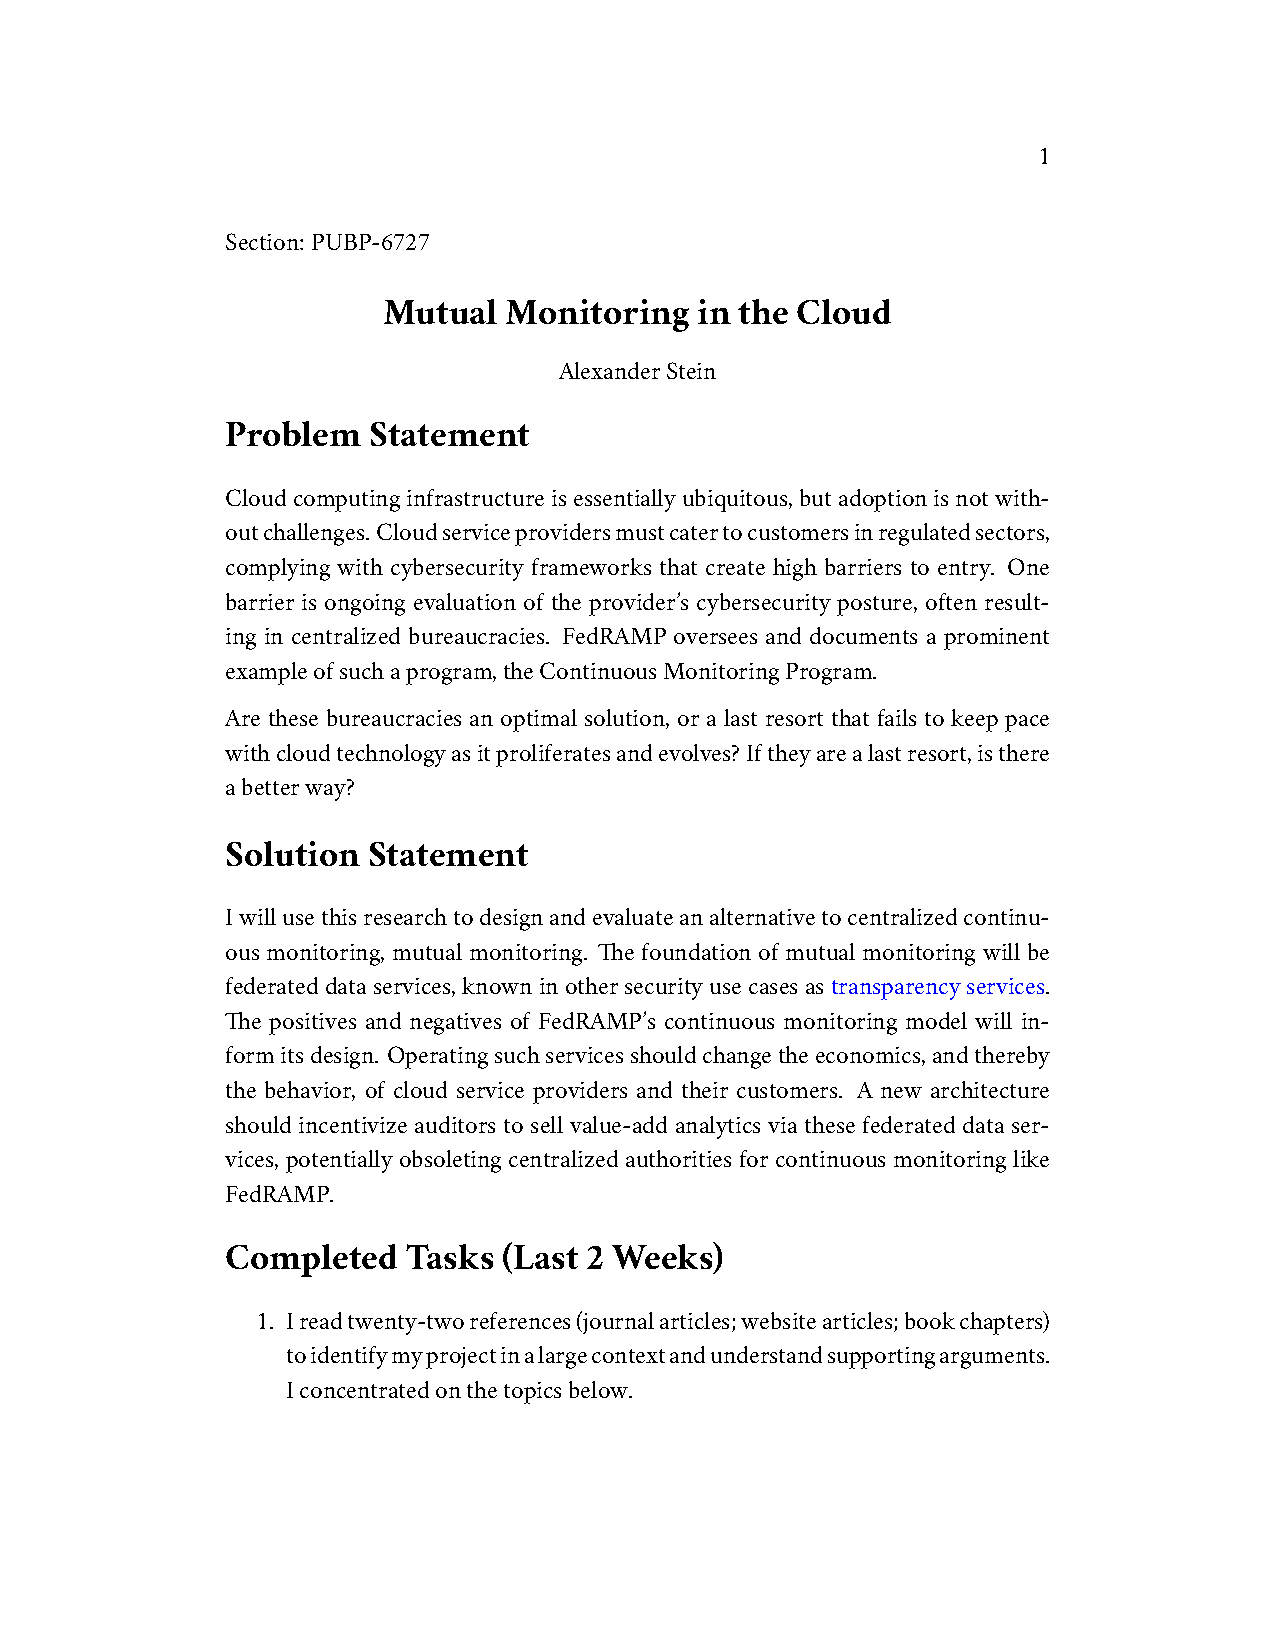
\includepdf[pages=-]{../proposal/paper.pdf}

\end{document}
